\documentclass[12pt]{article}

%configuraciones del idioma
\usepackage[spanish]{babel}
\usepackage[utf8]{inputenc}
\usepackage[T1]{fontenc}
\usepackage{bookman}

%cosas de matematicas
\usepackage{amsmath, amsfonts, amssymb}

%imagenes
\usepackage{graphicx}
\usepackage{subfigure} % subfiguras
\graphicspath{{imagenes/}}
\usepackage{float}

%dimensions
\usepackage[left=3.1cm, right=3.1cm, top=1.5cm]{geometry}

% para contraer referencias
\usepackage{url}
\usepackage{cite}

\usepackage[nottoc,numbib]{tocbibind}


\usepackage{color}
\definecolor{gray97}{gray}{.97}
\definecolor{gray75}{gray}{.75}
\definecolor{gray45}{gray}{.45}

%para escribir codigo
\usepackage{listings}

\lstset{ frame=Ltb,
framerule=0pt,
aboveskip=0.5cm,
framextopmargin=3pt,
framexbottommargin=3pt,
framexleftmargin=0.4cm,
framesep=0pt,
rulesep=.4pt,
backgroundcolor=\color{gray97},
rulesepcolor=\color{black},
%
stringstyle=\ttfamily,
showstringspaces = false,
basicstyle=\small\ttfamily,
commentstyle=\color{gray45},
keywordstyle=\bfseries,
%
numbers=left,
numbersep=15pt,
numberstyle=\tiny,
numberfirstline = false,
breaklines=true,
}

% minimizar fragmentado de listados
\lstnewenvironment{listing}[1][]
{\lstset{#1}\pagebreak[0]}{\pagebreak[0]}

\lstdefinestyle{consola}
{basicstyle=\scriptsize\bf\ttfamily,
backgroundcolor=\color{gray75},
}

\usepackage{charter} 

\title{Reporte práctica 2}
\author{Ian Mendoza Jaimes}
\date{}

\begin{document}

\begin{titlepage}
\centering
	\vspace*{1.5in}
	\begin{huge}
		Práctica 1\\
	\end{huge}
	\vspace{4em}
	\begin{Large}
		Ian Mendoza Jaimes \\
		\vspace{4em}
		Compiladores \\
		\vspace{1em}
		Profesor: Rafael Norman Saucedo Delgado \\
		\vspace{1em}
		Grupo: 3CM6 \\
		\vspace{1em}
	\end{Large}
\end{titlepage}

\tableofcontents
\pagenumbering{arabic}
\pagebreak

\section{Introducción}

Los autómatas al igual que las expresiones regulares son capaces de modelar lenguajes regulares. Estos lenguajes son particularmente útiles para describir algún lenguaje de programación. \\

Particularmente, los autómatas y las expresiones regulares son usados en la etapa del analisis léxico de un compilador \cite{automatas}. Primero se escriben expresiones regulares que describiran a las clases léxicas del lenguaje a traducir. Con estas expresiones, obtendremos sus respectivos autómtas. El problema, es que la construcción de Thompson arroja autómatas no deterministas, los cuales son más faciles de modelar, pero no de programar, además son más tardados de evaluar. \\

El tiempo de ejecución es muy importante en cualquier algoritmo, y el analizador léxico no es la excepción. Debido a que en esta etapa se evalua todo el código fuente de algún programa a traducir, puede tomar bastante tiempo. De ahi, surge la necesidad de utilizar autómtas deterministas para la obtención de tokens. \\

El algoritmo de los subconjuntos resuelve este problema \cite{compiladores}. Como entrada recibe un AFN y de salida arroja un AFD. Este método sin duda es uno de los más efectivos para la conversión de un AFN a un AFD, pues nos ahorra la necesidad de crear un AFN intermedio para lidear con las transiciones epsilon. \\

Antes de comenzar con la programación de este algoritmo, conviene describir las siguientes funciones auxiliares:

\begin{itemize}
	\item $Cerradura \epsilon (e)$, regresa todos los caminos que podemos seguir con una transición epsilon partiendo de algun estado dado $e$.
	\item $Mover(e,s)$, regresa los caminos que podemos seguir partiendo de un estado $e$ evaluando el caracter $s$.
\end{itemize}

El algoritmo de los subconjuntos consiste en los siguientes pasos:

\begin{enumerate}
	\item Agregar Cerradura $\epsilon$ (Inicial de AFN) a $E$
	\item Por cada estado $e \in E$
	\item 		Por cada símbolo $s$
	\item			Agregar Cerradura $\epsilon$ (Mover($e,s$))
	\item 			Agregar transición $E \xrightarrow[]{s} $ Cerradura $\epsilon$ (Mover($e,s$))
	\item El inicial del AFD es Cerradura $\epsilon$ (Inicial de AFN)
	\item Los finales del AFD contienen finales del AFN
\end{enumerate}











\newpage

\section{Desarrollo}

\subsection{Descripción de la problema}

Se deben implementar las clases Afn y Afd. Deben de permitir crear cualquier tipo de autómata y evaluar alguna cadena ingresada por el usuario.

\subsection{Código}

main.py
\lstset{language=Python, breaklines=true, basicstyle=\footnotesize}
\begin{lstlisting}[frame=single]
from afnd import Afn, Afd

class Main(object):

    def iniciar(self):
        automata = Afn()

        automata.anadirEstado()
        automata.anadirEstado()
        automata.anadirEstado()
        automata.anadirEstado()
        automata.anadirEstado()
        automata.anadirEstado()

        automata.anadirFinal(6)

        automata.anadirTransicion(1, 2, ['1'])
        automata.anadirTransicion(2, 1, ['1'])
        automata.anadirTransicion(2, 3, ['0'])
        automata.anadirTransicion(3, 2, ['0'])
        automata.anadirTransicion(3, 4, ['1'])
        automata.anadirTransicion(4, 3, ['1'])
        automata.anadirTransicion(4, 1, ['0'])
        automata.anadirTransicion(1, 4, ['0'])
        automata.anadirTransicion(4, 5)
        automata.anadirTransicion(5, 6, ['j'])

        for x in automata.crearTablaEstados():
            print(x)

        automata.dibujarAutomata()
        print('====')
        while True:
            print(automata.evaluarCadena(input("Ingresa una cadena: ")))
            if input("Quieres ingresar otra?: s/n    ") != 's':
                break


main = Main()
main.iniciar()
\end{lstlisting}

afnd.py
\lstset{language=Python, breaklines=true, basicstyle=\footnotesize}
\begin{lstlisting}[frame=single]
from estado import Estado, Transicion
import networkx as nx
import matplotlib.pyplot as plt

class Afn(object):

    def __init__(self):
        self.estados = []
        self.tablaEstados = []
        self.contadorEstados = 0
        self.inicial = 0
        self.historialCondiciones = set()
        self.err = 0

    def anadirEstado(self):
        self.contadorEstados += 1

        if self.inicial == 0:
            self.estados.append(Estado(self.contadorEstados, True))
            self.inicial = self.contadorEstados
        else:
            self.estados.append(Estado(self.contadorEstados, False))

        return self.contadorEstados

    def anadirTransicion(self, estado, siguiente, condiciones=[]):
        if estado > self.contadorEstados or estado < 1:
            return -1

        if siguiente > self.contadorEstados or estado < 1:
            return -1

        for x in condiciones:
            self.historialCondiciones.add(x)

        if len(condiciones) > 0:
            transicion = Transicion(siguiente, condiciones)
            self.estados[estado-1].anadirTransicion(transicion)
            for condicion in condiciones:
                self.historialCondiciones.add(condicion)
        else:
            transicion = Transicion(siguiente)
            self.estados[estado-1].anadirTransicion(transicion)

        return 0

    def anadirFinal(self, estado):
        if estado > self.contadorEstados or estado < 1:
            return -1

        self.estados[estado-1].volverFinal()
        return 0

    def cambiarInicial(self, estado):
        if estado > self.contadorEstados or estado < 1:
            return -1

        self.estados[self.inicial-1].volverInicial()
        self.estados[estado-1].volverInicial()
        self.inicial = estado
        return 0

    def dibujarAutomata(self):
        G = nx.DiGraph()
        etiqueta = {}
        for estado in self.estados:
            if estado.inicial:
                print('SOY EL INICIAL:', estado.nombre)
            if estado.final:
                print('SOY EL FINAL:', estado.nombre)
            for transicion in estado.transiciones:
                G.add_edge(estado.nombre, transicion.siguiente)
                etiqueta[estado.nombre, transicion.siguiente] = transicion.condiciones

        pos=nx.spring_layout(G)

        nx.draw_networkx_nodes(G, pos, node_size=500, node_color="blue")
        nx.draw_networkx_edges(G, pos,width=2, alpha=0.5, edge_color='black')
        nx.draw_networkx_labels(G, pos, font_size=5, font_family='sans-serif')

        nx.draw_networkx_edge_labels(G, pos, etiqueta, label_pos=0.3, with_labels = True)

        plt.show();

    def manejarEpsilon(self, nombreEstado):
        epsilons = self.estados[nombreEstado - 1].obtenerNumEpsilons()
        aux = [nombreEstado]

        if len(epsilons) == len(self.estados[nombreEstado - 1].transiciones) and len(self.estados[nombreEstado - 1].transiciones) > 0:
            aux.pop()
        if len(epsilons) == 0:
            return aux

        for e in epsilons:
            aux += self.manejarEpsilon(e)

        return aux


    def obtenerTransiciones(self, nombreEstado):
        aux = dict()
        aux[' '] = []
        for transicion in self.estados[nombreEstado - 1].transiciones:
            for condicion in transicion.condiciones:
                if condicion not in aux:
                    aux[condicion] = []

                aux[condicion].append(transicion.siguiente)

            if len(transicion.condiciones) == 0:
                aux[' '] += self.manejarEpsilon(transicion.siguiente)

        return aux


    def crearTablaEstados(self):
        if len(self.estados) == 0:
            return -1

        aux = []
        cont = 0
        for estado in self.estados:
            aux.append([])
            for condicion, etds in self.obtenerTransiciones(estado.nombre).items():
                if len(etds) > 0:
                    aux[cont].append([condicion, etds])
            cont += 1

        self.tablaEstados = aux
        return self.tablaEstados


    def validarCadena(self, cadena):
        if type(cadena) is not str:
            return False
        if len(self.tablaEstados) == 0:
            print(cadena)
        if type(self.inicial) is not int:
            return False

        return True


    def evaluarEpsilon(self, estados, caracter):
        temp = []
        for e in estados:
            for x in self.tablaEstados[e-1]:
                if x[0] == caracter:
                    temp += x[1]
                if x[0] == ' ':
                    temp += self.evaluarEpsilon(x[1], caracter)
        return temp


    def validacionFinal(self, estados):
        temp = []
        for e in estados:
            epsilons = self.estados[e-1].obtenerNumEpsilons()
            if len(epsilons) == 0:
                temp += [e]
            else:
                temp += self.validacionFinal(epsilons)
        return temp


    def evaluarCadena(self, cadena):
        if not self.validarCadena(cadena):
            return False

        if len(cadena) == 0:
            cadena = ' '

        estds = [self.inicial]
        temp = []
        temp2 = []

        for caracter in cadena:
            temp = []
            for e in estds:
                for x in self.tablaEstados[e-1]:
                    if x[0] == caracter:
                        temp += x[1]
                    if x[0] == ' ':
                        temp += self.evaluarEpsilon(x[1], caracter)
            estds = temp

        estds = self.validacionFinal(estds)

        for e in estds:
            if self.estados[e-1].final:
                return True

        return False


class Afd(Afn):

    def anadirTransicion(self, estado, siguiente, condiciones=[]):
        if len(condiciones) > 1:
            return -1

        if estado > self.contadorEstados or estado < 1:
            return -1

        if siguiente > self.contadorEstados or estado < 1:
            return -1

        if len(condiciones) > 0:
            transicion = Transicion(siguiente, condiciones)
            self.estados[estado-1].anadirTransicion(transicion)
        else:
            transicion = Transicion(siguiente)
            self.estados[estado-1].anadirTransicion(transicion)

        return 0
\end{lstlisting}

estado.py
\lstset{language=Python, breaklines=true, basicstyle=\footnotesize}
\begin{lstlisting}[frame=single]
class Transicion(object):
    def __init__(self, siguiente, condiciones=[]):
        self.condiciones = condiciones
        self.siguiente = siguiente


class Estado(object):
    def __init__(self, nombre, inicial=False, final=False):
        self.nombre = nombre
        self.inicial = inicial
        self.final = final
        self.transiciones = []

    def anadirTransicion(self, transicion):
        self.transiciones.append(transicion)
        return 0;

    def obtenerNumEpsilons(self):
        cont = []
        for t in self.transiciones:
            if len(t.condiciones) == 0:
                cont.append(t.siguiente)
        return cont

    def volverFinal(self):
        self.final = not self.final
        return 0;

    def volverInicial(self):
        self.inicial = not self.inicial
        return 0;
\end{lstlisting}


\newpage

\section{Resultados}

En esta sección se presentan capturas de pantallas de la ejecución del código presentado anteriormente.


\begin{figure}[H]
	\centering
	\subfigure[AFD obtenido de un AFN]{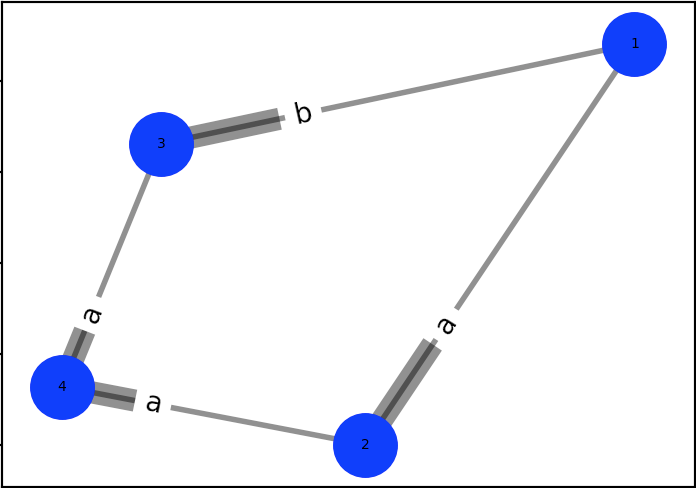
\includegraphics[width=12cm]{afd1}}
	\subfigure[Varias evaluaciones de cadenas]{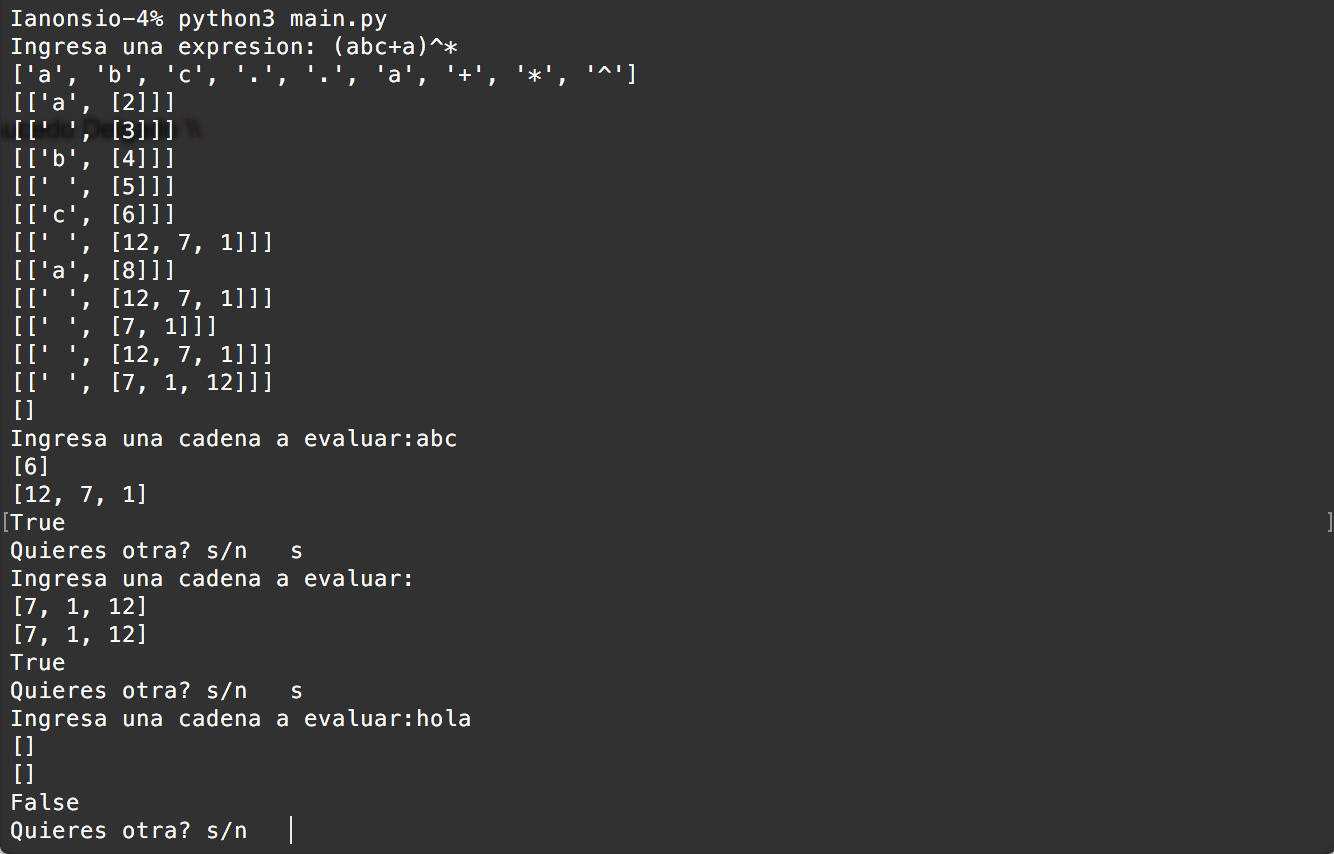
\includegraphics[width=12cm]{prueba1}}
	\caption{(a) El autómata generado por la expresión regular: $(a+b)a$. (b) El resultado de varias evaluaciones del autómata.}
	\label{fig:prueba1}
\end{figure}


\begin{figure}[H]
	\centering
	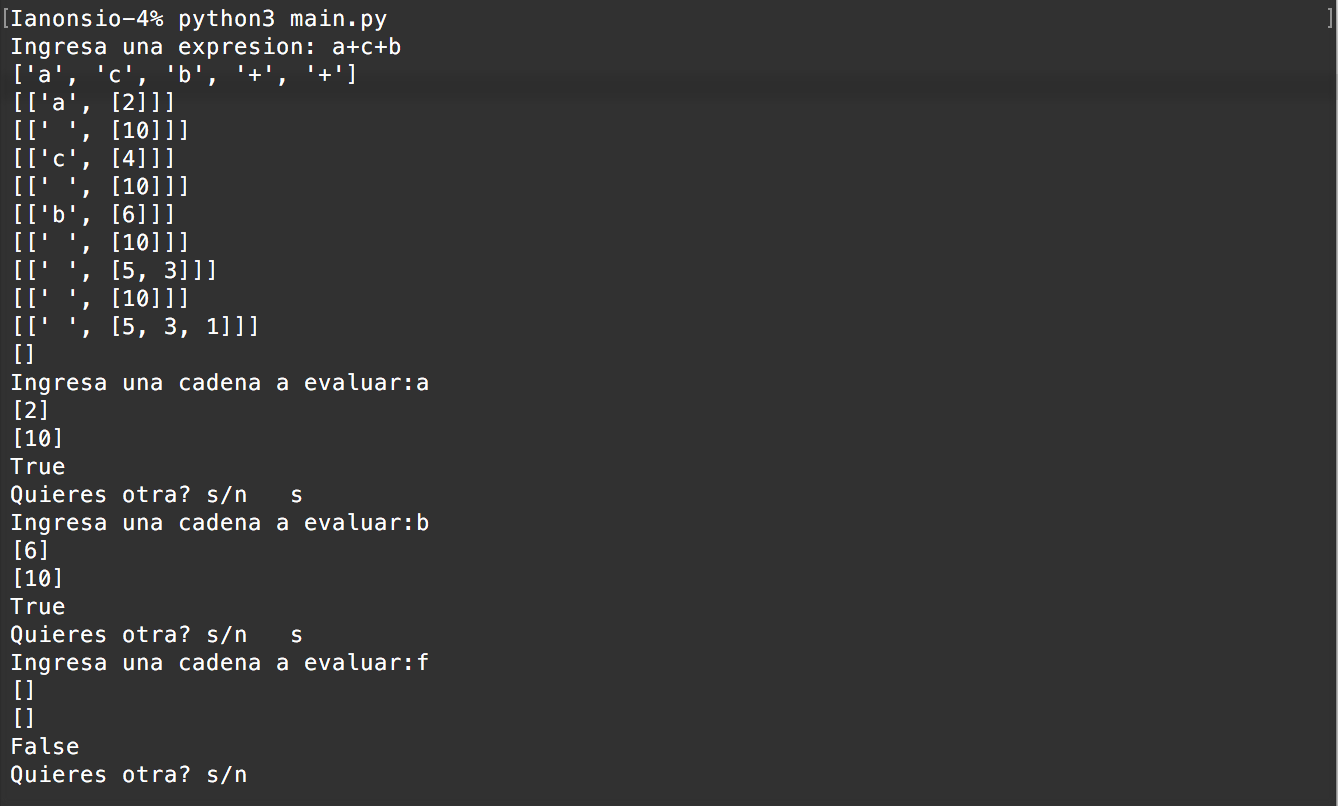
\includegraphics[width=12cm]{prueba2}
	\caption{Varias cadenas evaluadas con el autómata generado por la expresión regular: $(a+b)^{*}$.}
	\label{fig:prueba2}
\end{figure}














\newpage

\section{Conclusiones}

\vspace{3em}

\bibliographystyle{ieee}
\bibliography{bibliografia}

\end{document}